\documentclass[11pt,a4paper]{article}

% ---------------- PACKAGES ----------------
\usepackage[utf8]{inputenc}
\usepackage[T1]{fontenc}
\usepackage[english]{babel}
\usepackage{amsmath, amssymb}
\usepackage{siunitx}
\usepackage{geometry}
\usepackage{multicol}
\usepackage{tcolorbox}
\usepackage{tikz}
\usepackage{xcolor}
\usepackage{fancyhdr}

\geometry{margin=2cm}
\pagestyle{fancy}
\fancyhf{}
\lhead{\textbf{Power and Energy}}
\rhead{\thepage}

% ---------------- COLORS ----------------
\definecolor{energyblue}{RGB}{30,80,160}
\definecolor{powerred}{RGB}{180,50,50}
\definecolor{warningred}{RGB}{200,30,30}
\definecolor{graybg}{RGB}{245,245,245}

% ---------------- TCOLORBOX ----------------
\tcbset{
  sharp corners,
  colback=white,
  colframe=black!60,
  boxrule=0.8pt,
  left=6pt, right=6pt, top=4pt, bottom=4pt
}

\newcommand{\theorybox}[2]{
\begin{tcolorbox}[title=\textbf{#1}]
#2
\end{tcolorbox}
}

% ---------------- EXERCISE GRIDS ----------------
\newcommand{\fullgrid}{
\vfill
\begin{center}
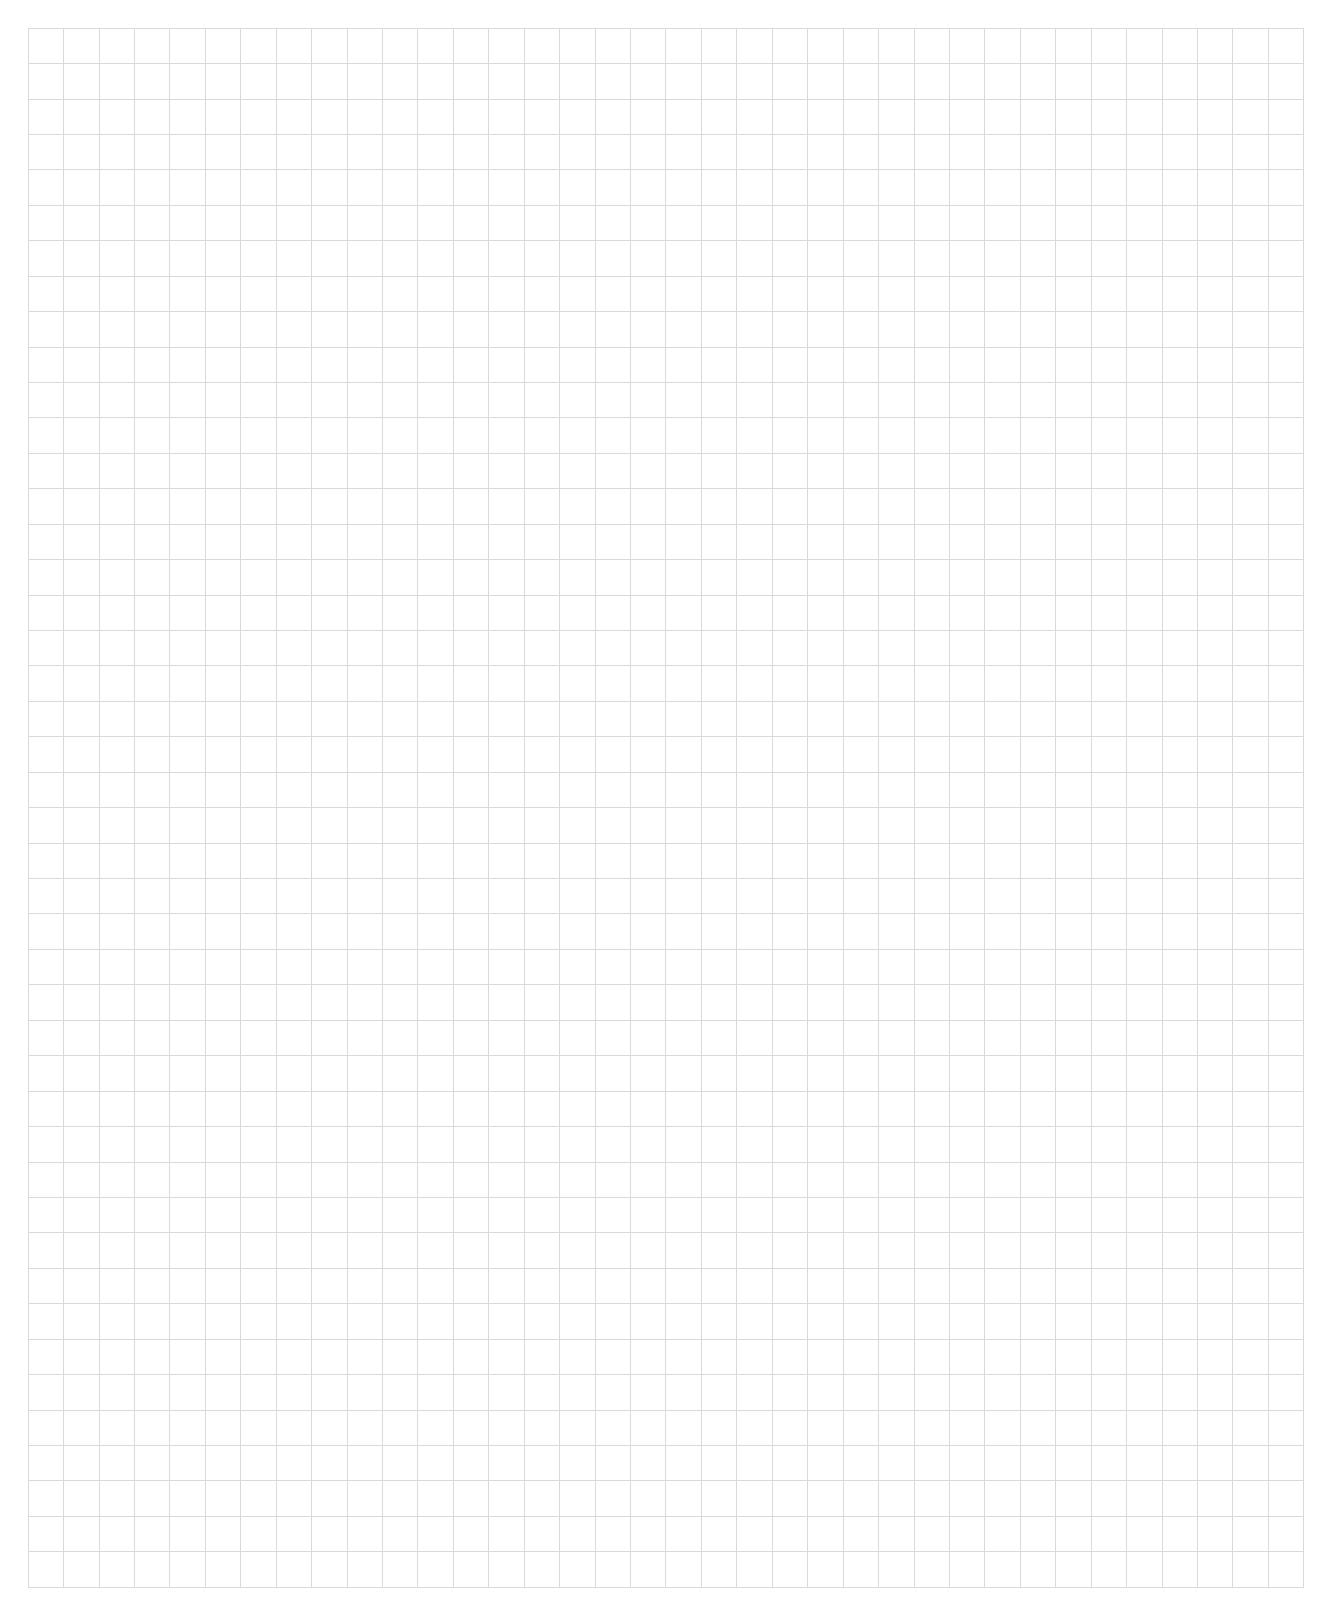
\begin{tikzpicture}[scale=0.9]
\draw[step=0.5cm,gray!30,very thin] (0,0) grid (18,22);
\end{tikzpicture}
\end{center}
\vfill
}

\newcommand{\threequartergrid}{
\vfill
\begin{center}

\begin{tikzpicture}[scale=0.9]
\draw[step=0.5cm,gray!30,very thin] (0,0) grid (18,18);
\end{tikzpicture}
\end{center}
\vfill
}

\begin{document}

% =================================================
% TITLE PAGE
% =================================================

\begin{center}
{\LARGE \textbf{Power and Energy}}\\[0.3cm]
{\large Basic reminders, SI units, conversions and exercises}\\[0.5cm]
\end{center}

% =================================================
% PART I : THEORY
% =================================================

\section*{I - Fundamental reminders}

% -------------------------------------------------
\theorybox{A - The 7 base units of the International System (SI)}{
The International System is based on \textbf{7 fundamental units}.  
All other units are built from them.

\begin{center}
\begin{tabular}{|c|c|c|}
\hline
\textbf{Quantity} & \textbf{Unit} & \textbf{Symbol} \\
\hline
Length & meter & m \\
Mass & kilogram & kg \\
Time & second & s \\
Electric current & ampere & A \\
Temperature & kelvin & K \\
Amount of substance & mole & mol \\
Luminous intensity & candela & cd \\
\hline
\end{tabular}
\end{center}
}

% -------------------------------------------------
\theorybox{B - Common derived units}{
Derived units are combinations of SI base units.

\begin{itemize}
\item Distance: cm, km (but \textbf{the SI unit is the meter})
\item Mass: g, ton (but \textbf{the SI unit is the kilogram})
\item Volume: liter (L), m$^3$ (\textbf{always convert to m$^3$})
\item Speed: m/s, km/h
\item Energy: joule (J)
\item Temperature: °C (warning: SI unit is kelvin)
\item Electric charge: coulomb (C) / ampere-hour (Ah)
\item Electric potential: volt (V)
\end{itemize}

Examples of conversions and relations:
\[
1\,\si{L} = 10^{-3}\,\si{m^3}
\qquad
1\,\si{km/h} = \frac{1000}{3600}\,\si{m/s}
\]

Electrical relations:
\[
1\,\si{C} = 1\,\si{A} \cdot 1\,\si{s}
\qquad
1\,\si{V} = 1\,\frac{\si{J}}{\si{C}} = 1\,\frac{kg \cdot m^2}{s^3 \cdot A}
\qquad
1\,\si{Ah} = 3600\,\si{C}
\]
}

% -------------------------------------------------
\theorybox{C - ABSOLUTE RULE - SI UNITS}{
\centering
\textbf{\Large EVERYTHING MUST BE IN SI UNITS BEFORE USING A FORMULA}

\vspace{0.2cm}

No grams.  
No tons.  
No kilometers.  
No centimeters.  

\textbf{kg, m, s, A, K.}

Otherwise, \textbf{the result is wrong}, even if the math is correct.
}

% -------------------------------------------------
\theorybox{D - Decimal conversion (lengths, masses)}{
For lengths and masses, we use a \textbf{decimal conversion table}.

Example: Conversion of $1470\,\si{mm}$ into meters  
\textbf{Conversion table:}

\begin{center}
\begin{tabular}{c|c|c|c|c|c|c}
km & hm & dam & m & dm & cm & mm \\
\hline
   &    &     & 1 & 4  & 7  & 0  \\
\end{tabular}
\end{center}

Each shift one column to the left corresponds to a division by 10.

\vspace{0.2cm}

\textbf{Decimal writing with decimal point shift:}

\[
1470\,\si{mm}
\;\longrightarrow\;
147.\!0\,\si{cm}
\;\longrightarrow\;
14.\!70\,\si{dm}
\;\longrightarrow\;
1.\!470\,\si{m}
\]

\vspace{0.2cm}

\textbf{Final result:}

\[
1470\,\si{mm} = 1.47\,\si{m}
\]

Each shift to the right multiplies by 10.  
Each shift to the left divides by 10.

Example:
\[
250\,\si{cm} = 2.5\,\si{m}
\qquad
3.2\,\si{km} = 3200\,\si{m}
\]
}

% -------------------------------------------------
\theorybox{E - Area and volume conversions (dimensional table)}{

\textbf{Visual principle:}

\begin{itemize}
\item Area $\rightarrow$ two dimensions $\rightarrow$ \textbf{two zeros}
\item Volume $\rightarrow$ three dimensions $\rightarrow$ \textbf{three zeros}
\end{itemize}

\vspace{0.2cm}

\textbf{Example - Converting $25\,\si{cm^2}$ to $\si{m^2}$}

\begin{center}
\textbf{Area table}
\begin{tabular}{c|c|c|c|c|c|c}
km$^2$ & hm$^2$ & dam$^2$ & m$^2$ & dm$^2$ & cm$^2$ & mm$^2$ \\
\hline
       &        &         & 0 0 & 2 5 &       &        \\
\end{tabular}
\end{center}

Table reading:
\[
25\,\si{cm^2} = 0.0025\,\si{m^2}
\]

\[
25\,\si{cm^2} = 2.5 \times 10^{-3}\,\si{m^2}
\]

\vspace{0.4cm}

\textbf{Example - Converting $4\,\si{cm^3}$ to $\si{m^3}$}

\begin{center}
\textbf{Volume table}
\begin{tabular}{c|c|c|c|c|c|c}
km$^3$ & hm$^3$ & dam$^3$ & m$^3$ & dm$^3$ & cm$^3$ & mm$^3$ \\
\hline
       &        &         & 0 0 0 & 0 0 4 &        &        \\
\end{tabular}
\end{center}

Table reading:
\[
4\,\si{cm^3} = 0.000004\,\si{m^3}
\]

\[
4\,\si{cm^3} = 4 \times 10^{-6}\,\si{m^3}
\]

\vspace{0.2cm}

\textbf{Key message:}

Zeros are not decorative.  
They encode the \textbf{number of dimensions}.
}

% -------------------------------------------------
\theorybox{F - Conversion by proportion (general case)}{
When conversion is not decimal, use a \textbf{proportion}.

Examples:

\[
1\,\text{lb} = 453\,\si{g}
\Rightarrow
5\,\text{lb} = 5 \times 0.453 = 2.27\,\si{kg}
\]

\[
1\,\si{km/h} = \frac{1000}{3600}\,\si{m/s}
\Rightarrow
120\,\si{km/h} = 33.3\,\si{m/s}
\]
}

% -------------------------------------------------
\theorybox{G - Definition of energy (physical intuition)}{
Energy is not directly visible, but it is \textbf{felt} when effort is required.

\textbf{Example: The bicycle and the hill}

To climb, the cyclist must \textbf{exert effort}.  
That energy is stored as \textbf{gravitational potential energy}:

\[
E_p = m g h
\]

Arriving at the top, the bike is motionless, but the energy is still there.

Descending, that energy becomes \textbf{kinetic energy}:

\[
E_c = \frac{1}{2} m v^2
\]

\textbf{Key idea:}

Energy does not disappear.  
It \textbf{changes form}.

\[
E_p \longrightarrow E_c
\]

All energies are measured in \textbf{joules}:

\[
[J] = kg \cdot m^2 \cdot s^{-2}
\]
}

% -------------------------------------------------
\theorybox{H - Definition of power (physical intuition)}{
Power measures the \textbf{rate at which energy is transferred}.

\[
P = \frac{E}{t}
\qquad
1\,\si{W} = 1\,\si{J/s}
\]

Same energy, different power $\Rightarrow$ different time.

\[
t = \frac{E}{P}
\]

Power is an \textbf{energy flow rate}.
}

% -------------------------------------------------
\theorybox{I - Dimensional analysis (unit signature)}{
Each unit has a \textbf{unique signature}, like a factorization into prime numbers.

\[
J = kg \cdot m^2 \cdot s^{-2}
\]

If the units do not match, the result \textbf{is not an energy}.  

Example:
\[
E = m[kg]\cdot g[ms^{-2}]\cdot h[m]
\Rightarrow
kg \times \frac{m}{s^2} \times m = kg \cdot m^2 \cdot s^{-2}
\]

Dimensional analysis is an \textbf{error-detection tool}.
}

% -------------------------------------------------
\theorybox{J - Common energy and power formulas}{
All energies have signature $kg \cdot m^2 \cdot s^{-2}$  
All powers have signature $kg \cdot m^2 \cdot s^{-3}$


\textbf{Energy}

\begin{center}
\begin{tabular}{|>{\small}l|>{\small}l|>{\small}l|>{\small}l|}
\hline
\textbf{Nom} & \textbf{Formule} & \textbf{Paramètres} & \textbf{Signature SI} \\
\hline
Potentielle (gravité) & $E_p = m g h$ & $m$ masse [kg], $g$ gravité [m/s²], $h$ hauteur [m] & $kg \cdot m^2 \cdot s^{-2}$ \\
\hline
Cinétique & $E_c = \frac{1}{2} m v^2$ & $m$ masse [kg], $v$ vitesse [m/s] & $kg \cdot m^2 \cdot s^{-2}$ \\
\hline
Thermique & $E_{th} = m c \Delta T$ & $m$ masse [kg], $c$ chaleur spé... [J/kg·K], $\Delta T$ [K] & $kg \cdot m^2 \cdot s^{-2}$ \\
\hline
Travail d'une force & $W = F d$ & $F$ force [N], $d$ distance [m] & $kg \cdot m^2 \cdot s^{-2}$ \\
\hline
Électrique & $E = U I t$ & $U$ tension [V], $I$ courant [A], $t$ durée [s] & $kg \cdot m^2 \cdot s^{-2}$ \\
\hline
Changement d'état & $E_\text{ch} = m L$ & $m$ masse [kg], $L$ chaleur latente [J/kg] & $kg \cdot m^2 \cdot s^{-2}$ \\
\hline
\end{tabular}
\end{center}

\vspace{0.3cm}

\textbf{Power}

\begin{center}
\begin{tabular}{|l|l|l|l|}
\hline
\textbf{Nom} & \textbf{Formule} & \textbf{Paramètres} & \textbf{Signature SI} \\
\hline
Générale & $P = \frac{E}{t}$ & $E$ énergie [J], $t$ temps [s] & $kg \cdot m^2 \cdot s^{-3}$ \\
\hline
Mécanique (force) & $P = F v$ & $F$ force [N], $v$ vitesse [m/s] & $kg \cdot m^2 \cdot s^{-3}$ \\
\hline
Électrique & $P = U I$ & $U$ tension [V], $I$ courant [A] & $kg \cdot m^2 \cdot s^{-3}$ \\
\hline
\end{tabular}
\end{center}

}

% =================================================
% PART II : EXERCISES
% =================================================

\newpage
\section*{II - Exercises}


% -------------------------------------------------
\subsection*{Exercise 1 - Train and potential energy}

A train of mass $400\,\si{t}$ climbs a hill of $80\,\si{m}$.

\begin{itemize}
\item Draw a diagram of the situation with the known data.
\item Convert all data into SI units.
\item Calculate the potential energy gained.
\end{itemize}

\fullgrid

% -------------------------------------------------
\newpage
\subsection*{Exercise 2 - Kinetic energy of a car}

A car of mass $1200\,\si{kg}$ is driving at $120\,\si{km/h}$.

\begin{itemize}
\item Draw a diagram of the situation with the known data.
\item Convert the speed into m/s.
\item Calculate the kinetic energy.
\end{itemize}

\fullgrid

% -------------------------------------------------
\newpage
\subsection*{Exercise 3 - Bicycle downhill}

A 100 kg bicycle descends a hill of height $25\,\si{m}$.  
Calculate the speed at the bottom of the hill in km/h.  
Friction will be neglected.

\begin{itemize}
\item Draw a diagram of the situation with the known data.
\item Calculate the energy.
\item Calculate the speed at the bottom of the hill.
\item Convert the speed into the requested unit.
\end{itemize}

\fullgrid

% -------------------------------------------------
\newpage
\subsection*{Exercise 4 - Bicycle uphill}

A bicycle reaches the bottom of a hill with a speed of $120\,\si{km/h}$.  
What is the height of the hill, knowing that the bicycle slows down while climbing and comes to rest exactly at the top?

\begin{itemize}
\item Draw a diagram of the situation with the known data.
\item Convert the speed into m/s.
\item Calculate the energy.
\item Calculate the height.
\end{itemize}

\fullgrid

% -------------------------------------------------
\newpage
\subsection*{Exercise 5 - Elevator}

An elevator with a total mass of $900\,\si{kg}$ is pulled by a $1000\,\si{W}$ motor and must climb a tower of $120\,\si{m}$.

\begin{itemize}
\item Draw a diagram of the situation with the known data.
\item Calculate the total energy.
\item Calculate the ascent time using the power.
\end{itemize}

\fullgrid

% -------------------------------------------------
\newpage
\subsection*{Exercise 6 - Hydroelectric dam}

A dam lets $2000\,\si{kg/s}$ of water flow from a height of $600\,\si{m}$.  
The lake measures $2\,\si{km} \times 5\,\si{km}$ and is $50\,\si{m}$ deep.  
The depth of the lake is neglected for the calculation.  
Use only the penstock height of $600\,\si{m}$.

Calculate the maximum power the dam can deliver in kilowatts, as well as the total energy stored in the lake in kilowatt-hours.

\begin{itemize}
\item Draw a diagram of the situation with the known data.
\item Convert all quantities into SI units.
\item Calculate the power.
\item Calculate the energy stored in the lake.
\end{itemize}

\threequartergrid

% -------------------------------------------------
\newpage
\subsection*{Exercise 7 - Battery}

A battery supplies $24\,\si{V}$ and $15\,\si{A}$ for $3\,\si{h}$.  
Calculate the power, then calculate the total energy in joules and in watt-hours.

\begin{itemize}
\item Draw a diagram of the situation with the known data.
\item Convert all quantities into SI units.
\item Calculate the power.
\item Calculate the energy in joules.
\item Convert the energy into Wh.
\end{itemize}

\threequartergrid

% -------------------------------------------------
\newpage
\subsection*{Exercise 8 - Heater}

A $2000\,\si{W}$ heater operates for $45\,\si{min}$.

\begin{itemize}
\item Draw a diagram of the situation with the known data.
\item Convert all quantities into SI units.
\item Calculate the energy consumed.
\end{itemize}

\fullgrid

% -------------------------------------------------
\newpage
\subsection*{Exercise 9 - Vertical jump}

A $70\,\si{kg}$ person jumps vertically to a height of $40\,\si{cm}$.  
What is their speed just before touching the ground on the way down?

\begin{itemize}
\item Draw a diagram of the situation with the known data.
\item Convert all quantities into SI units.
\item Calculate the potential energy.
\item Deduce the speed.
\end{itemize}

\fullgrid

% -------------------------------------------------
\newpage
\subsection*{Exercise 10 - Turbine}

A turbine receives $30'000\,\si{liters/s}$ of water from a height of $25\,\si{m}$.  
What is the theoretical power available on the turbine shaft?

\begin{itemize}
\item Draw a diagram of the situation with the known data.
\item Convert all quantities into SI units.
\item Calculate the power.
\end{itemize}

\fullgrid

% -------------------------------------------------
\newpage
\subsection*{Exercise 12 - Solar panel}

Solar panels with a surface area of $12\,\si{m^2}$ are exposed to intense sunlight  
(clear weather, sun high in the sky).

The solar irradiance at ground level is $I = 1000\,\si{W/m^2}$ and the panel has an efficiency of $25\%$.  

Calculate the electrical power available at the panel output in [W], as well as the total electrical energy produced between 11 a.m. and 1 p.m. in [kWh].

Reminder: An efficiency of $25\%$ means that \textbf{only one quarter} of the incoming light energy is converted into electricity.  
The rest is mainly lost as heat.

\begin{itemize}
\item Draw a simple diagram of the panel and the solar radiation.
\item Identify the known data and their units.
\item Calculate the solar power received by the panel.
\item Calculate the available electrical power, taking efficiency into account.
\item Calculate the energy produced.
\end{itemize}

\threequartergrid

% -------------------------------------------------
\newpage
\subsection*{Exercise 13 - Kettles and power}

Two electric kettles are used to heat water:

\begin{itemize}
\item Kettle A: $100\,\si{ml}$ of water at $50\,\si{°C}$ with a power of $100\,\si{W}$.
\item Kettle B: $1.5\,\si{L}$ of water at $20\,\si{°C}$ with a power of $2000\,\si{W}$.
\end{itemize}

The specific heat capacity of water is  
\[
c = 4180\,\si{J/(kg \cdot K)}
\]

\textbf{Question:} Which of the two kettles will bring its water to $100\,\si{°C}$ first, and how long will it take for each one?

\begin{itemize}
\item Draw a diagram of the situation with the known data.
\item Convert all data into SI units.
\item Calculate the required energy for each case.
\item Calculate the time using the power.
\end{itemize}

\threequartergrid

\end{document}

